\documentclass[12pt,twoside,a4paper]{article}

\textwidth 17cm \textheight 25cm \evensidemargin 0cm
\oddsidemargin 0cm \topmargin -2cm
\parindent 0pt
%\parskip \bigskipamount

\usepackage{graphicx}
\usepackage[dutch]{babel}
\usepackage{amssymb,amsthm,amsmath}
%\usepackage{dot2texi}
\usepackage[utf8]{inputenc}
\usepackage{nopageno}
\usepackage{pdfpages}
\usepackage{enumerate}
\usepackage{caption}
\usepackage{wrapfig}
\usepackage{pgf,tikz,pgfplots}
\pgfplotsset{compat=1.15}
\usepackage{color}
\usetikzlibrary{arrows}
\usetikzlibrary{patterns}
\usepackage{fancyhdr}
\pagestyle{fancy}
\usepackage[version=3]{mhchem}
\usepackage{multicol}
\usepackage{fix-cm}
\usepackage{setspace}
\usepackage{mhchem}
\usepackage{xhfill}
\usepackage{parskip}
\usepackage{cancel}
\usepackage{mdframed}
\usepackage{url}
\usepackage{mathtools}
\usepackage{changepage}

\newcommand{\todo}[1]{{\color{red} TODO: #1}}

\newcommand{\degree}{\ensuremath{^\circ}}
\newcommand\rad{\qopname\relax o{\mathrm{rad}}}

\newcommand\ggd{\qopname\relax o{\mathrm{ggd}}}

\pgfmathdeclarefunction{gauss}{2}{%
  \pgfmathparse{1/(#2*sqrt(2*pi))*exp(-((x-#1)^2)/(2*#2^2))}%
}

\def\LRA{\Leftrightarrow}

\newcommand{\zrmbox}{\framebox{\phantom{EXE}}\phantom{X}}
\newcommand{\zrm}[1]{\framebox{#1}}

% environment oefening:
% houdt een teller bij die de oefeningen nummert, probeert ook de oefening op één pagina te houden
\newcounter{noefening}
\setcounter{noefening}{0}
\newenvironment{oefening}
{
  \stepcounter{noefening}
  \pagebreak[0]
  \begin{minipage}{\textwidth}
  \vspace*{0.7cm}{\large\bf Oefening \arabic{noefening}}
}{%
  \end{minipage}
}

\usepackage{calc}

% vraag
\reversemarginpar
\newcounter{punten}
\setcounter{punten}{0}
\newcounter{nvraag}
\setcounter{nvraag}{1}
\newlength{\puntwidth}
\newlength{\boxwidth}
\newcommand{\vraag}[1]{
\settowidth{\puntwidth}{\Large{#1}}
\setlength{\boxwidth}{1.5cm}
\addtolength{\boxwidth}{-\puntwidth}
{\large\bf Vraag \arabic{nvraag} \addtocounter{nvraag}{1}}\vspace*{-0.5cm}
{\marginpar{\color{lightgray}\fbox{\parbox{1.5cm}{\vspace*{1cm}\hspace*{\boxwidth}{\Large{#1}}}}}
\vspace*{0.5cm}}
\addtocounter{punten}{#1}}

% arulefill
\def\arulefill{\leavevmode{\xrfill[-5pt]{0.3pt}[lightgray]\endgraf}\vspace*{0.2cm}}

% \arules{n}
\newcommand{\arules}[1]{
\color{lightgray}
%\vspace*{0.05cm}
\foreach \n in {1,...,#1}{
  \vspace*{0.75cm}
  \hrule height 0.3pt\hfill
}\color{black}\vspace*{0.2cm}}

% \arule{x}
\newcommand{\arule}[1]{
\color{lightgray}{\raisebox{-0.1cm}{\rule[-0.05cm]{#1}{0.3pt}}}\color{black}
}

% \abox{y}
\newcommand{\abox}[1]{
\fbox{
\begin{minipage}{\textwidth- 4\fboxsep}
\hspace*{\textwidth}\vspace{#1}
\end{minipage}
}
}

\newcommand{\ruitjes}[1]{
\definecolor{cqcqcq}{rgb}{0.85,0.85,0.85}
\hspace*{-2.5cm}
\begin{tikzpicture}[scale=1.04,line cap=round,line join=round,>=triangle 45,x=1.0cm,y=1.0cm]
\draw [color=cqcqcq, xstep=0.5cm, ystep=0.5cm] (0,-#1) grid (20.5,0);
\end{tikzpicture}
}


\newcommand{\assenstelsel}[5][1]{
\definecolor{cqcqcq}{rgb}{0.65,0.65,0.65}
\begin{tikzpicture}[line cap=round,line join=round,>=triangle 45,x=#1cm,y=#1cm]
\draw [color=cqcqcq,dash pattern=on 1pt off 1pt, xstep=1.0cm,ystep=1.0cm] (#2,#4) grid (#3,#5);
\draw[->,color=black] (#2,0) -- (#3,0);
%\draw[shift={(1,0)},color=black] (0pt,2pt) -- (0pt,-2pt) node[below] {\footnotesize $1$};
%\draw[color=black] (#3.25,0.07) node [anchor=south west] {$x$};
\draw[->,color=black] (0,#4) -- (0,#5);
%\draw[shift={(0,1)},color=black] (2pt,0pt) -- (-2pt,0pt) node[left] {\footnotesize $1$};
\draw[color=black] (0.09,#5.25) node [anchor=west] {\phantom{$y$}};
%\draw[color=black] (0pt,-10pt) node[right] {\footnotesize $0$};
\end{tikzpicture}
}

\newcommand{\getallenas}[3][1]{
\definecolor{cqcqcq}{rgb}{0.65,0.65,0.65}
\begin{tikzpicture}[scale=#1,line cap=round,line join=round,>=triangle 45,x=1.0cm,y=1.0cm]
\draw [color=cqcqcq,dash pattern=on 1pt off 1pt, xstep=1.0cm,ystep=1.0cm] (#2,-0.2) grid (#3,0.2);
\draw[->,color=black] (#2.25,0) -- (#3.5,0);
\draw[shift={(0,0)},color=black] (0pt,2pt) -- (0pt,-2pt) node[below] {\footnotesize $0$};
\draw[shift={(1,0)},color=black] (0pt,2pt) -- (0pt,-2pt) node[below] {\footnotesize $1$};
\draw[color=black] (#3.25,0.07) node [anchor=south west] {$\mathbb{R}$};
\end{tikzpicture}
}

\newcommand{\visgraad}[1]{\begin{tabular}{p{0.5cm}|p{#1}}&\\\hline\\\end{tabular}}

\newcommand{\tekenschema}[2]{\begin{tabular}{p{0.5cm}|p{#1}}&\\\hline\\[#2]\end{tabular}}

% schema van Horner
\newcommand{\schemahorner}{
\begin{tabular}{p{0.5cm}|p{7cm}}
&\\[1.5cm]
\hline\\
\end{tabular}}

% geef tabular iets meer ruimte
\setlength{\tabcolsep}{14pt}
\renewcommand{\arraystretch}{1.5}

\newcommand{\toets}[3]{
\thispagestyle{plain}
\vspace*{-2.5cm}
\begin{tikzpicture}[remember picture, overlay]
    \node [shift={(15.25 cm,-1.6cm)}] {%
        \includegraphics[width=1.8cm]{/home/ppareit/kaa1415/logokaavelgem.png}%
    };%
\end{tikzpicture}

\begin{tabular}{|llc|c|}
\hline
\vspace*{-0.5cm}
&&&\\
Naam & \arule{4cm} & {\Large\bf KA AVELGEM} & \\
\vspace*{-0.75cm}
&&&\\
Klas & \arule{4cm} & {\Large\bf 20...-...-...} & \\
\hline
\vspace*{-0.75cm}
&&&\\
Toets & {\bf #2} & {\large\bf #1} & Beoordeling\\
\vspace*{-0.75cm}
&&&\\
Onderwerp & \multicolumn{2}{l|}{\bf #3} &\\
\hline
\end{tabular}
}

\newcommand{\oefeningen}[1]{

\fancyhead[LE, RO]{\vspace{0.5cm} #1}
%\thispagestyle{plain}

{\bf \Large \centering Oefeningen: #1}

}

\raggedbottom

\newcommand\vl{\qopname\relax o{\mathrm{vl}}}

\newcommand\dom{\qopname\relax o{\mathrm{dom}}}
\newcommand\ber{\qopname\relax o{\mathrm{ber}}}

\newcommand\mC{\qopname\relax o{\mathrm{mC}}}
\newcommand\uC{\qopname\relax o{\mathrm{{\mu}C}}}
\newcommand\C{\qopname\relax o{\mathrm{C}}}

\newcommand\W{\qopname\relax o{\mathrm{W}}}
\newcommand\kW{\qopname\relax o{\mathrm{kW}}}
\newcommand\kWh{\qopname\relax o{\mathrm{kWh}}}


\newcommand\V{\qopname\relax o{\mathrm{V}}}
\newcommand\ohm{\qopname\relax o{\mathrm{\Omega}}}
\newcommand\kohm{\qopname\relax o{\mathrm{k\Omega}}}


\newcommand\N{\qopname\relax o{\mathrm{N}}}

\newcommand\Nperkg{\qopname\relax o{\mathrm{N/kg}}}

\newcommand\Nperm{\qopname\relax o{\mathrm{N/m}}}

\newcommand\gpermol{\qopname\relax o{\mathrm{g/mol}}}


\newcommand\kgperm{\qopname\relax o{\mathrm{kg/m}}}
\newcommand\kgperdm{\qopname\relax o{\mathrm{kg/dm}}}
\newcommand\gpercm{\qopname\relax o{\mathrm{g/cm}}}
\newcommand\gperml{\qopname\relax o{\mathrm{g/ml}}}


\newcommand{\mA}{\;\mbox{mA}}
\newcommand{\A}{\;\mbox{A}}
\newcommand{\MA}{\;\mbox{MA}}

\newcommand{\us}{\;\mu\mbox{s}}
\newcommand\s{\qopname\relax o{\mathrm{s}}}

\newcommand\h{\qopname\relax o{\mathrm{h}}}

\newcommand{\kmperh}{\;\mbox{km/h}}
\newcommand{\mpers}{\;\mbox{m/s}}
\newcommand{\kmpermin}{\;\mbox{km/min}}
\newcommand{\kmpers}{\;\mbox{km/s}}

\newcommand{\mph}{\;\mbox{mph}}

\newcommand{\Hz}{\;\mbox{Hz}}

\newcommand\Gm{\qopname\relax o{\mathrm{Gm}}}
\newcommand\Mm{\qopname\relax o{\mathrm{Mm}}}
\newcommand\km{\qopname\relax o{\mathrm{km}}}
\newcommand\hm{\qopname\relax o{\mathrm{hm}}}
\newcommand\dam{\qopname\relax o{\mathrm{dam}}}
\newcommand\m{\qopname\relax o{\mathrm{m}}}
\newcommand\dm{\qopname\relax o{\mathrm{dm}}}
\newcommand\cm{\qopname\relax o{\mathrm{cm}}}
\newcommand\mm{\qopname\relax o{\mathrm{mm}}}
\newcommand\um{\qopname\relax o{\mathrm{{\mu}m}}}
\newcommand\nm{\qopname\relax o{\mathrm{nm}}}


\newcommand\Gg{\qopname\relax o{\mathrm{Gg}}}
\newcommand\Mg{\qopname\relax o{\mathrm{Mg}}}
\newcommand\kg{\qopname\relax o{\mathrm{kg}}}
\newcommand\hg{\qopname\relax o{\mathrm{hg}}}
\renewcommand\dag{\qopname\relax o{\mathrm{dag}}}
\newcommand\g{\qopname\relax o{\mathrm{g}}}
\newcommand\dg{\qopname\relax o{\mathrm{dg}}}
\newcommand\cg{\qopname\relax o{\mathrm{cg}}}
\newcommand\mg{\qopname\relax o{\mathrm{mg}}}
\newcommand\ug{\qopname\relax o{\mathrm{{\mu}g}}}
\renewcommand\ng{\qopname\relax o{\mathrm{ng}}}

\newcommand\ton{\qopname\relax o{\mathrm{ton}}}

\newcommand\Gl{\qopname\relax o{\mathrm{Gl}}}
\newcommand\Ml{\qopname\relax o{\mathrm{Ml}}}
\newcommand\kl{\qopname\relax o{\mathrm{kl}}}
\newcommand\hl{\qopname\relax o{\mathrm{hl}}}
\newcommand\dal{\qopname\relax o{\mathrm{dal}}}
\renewcommand\l{\qopname\relax o{\mathrm{l}}}
\newcommand\dl{\qopname\relax o{\mathrm{dl}}}
\newcommand\cl{\qopname\relax o{\mathrm{cl}}}
\newcommand\ml{\qopname\relax o{\mathrm{ml}}}
\newcommand\ul{\qopname\relax o{\mathrm{{\mu}l}}}
\newcommand\nl{\qopname\relax o{\mathrm{nl}}}

\newcommand\MJ{\qopname\relax o{\mathrm{MJ}}}
\newcommand\kJ{\qopname\relax o{\mathrm{kJ}}}
\newcommand\J{\qopname\relax o{\mathrm{J}}}

\newcommand\T{\qopname\relax o{\mathrm{T}}}
\newcommand\uT{\qopname\relax o{\mathrm{{\mu}T}}}

\newcommand\grC{\qopname\relax o{\mathrm{{\degree}C}}}

\newcommand\K{\qopname\relax o{\mathrm{K}}}
\newcommand\calperK{\qopname\relax o{\mathrm{cal/K}}}

\newcommand\hPa{\qopname\relax o{\mathrm{hPa}}}
\newcommand\Pa{\qopname\relax o{\mathrm{Pa}}}

\newcommand\dB{\qopname\relax o{\mathrm{dB}}}

\newcommand\Var{\qopname\relax o{\mathrm{Var}}}

\newcommand{\EE}[1]{\cdot 10^{#1}}

\onehalfspacing

%\setlength{\headsep}{0cm}

\newenvironment{exlist}[1] %
{ \begin{multicols}{#1}
  \begin{enumerate}[(a)]
    \setlength{\itemsep}{0.5em} }
{ \end{enumerate}
  \end{multicols} }




\begin{document}

\begin{center}
  \begin{mdframed}
    \centering
    \fontsize{40}{60}\selectfont Complexe Getallen
  \end{mdframed}
  \vspace*{2.5cm}
  \begin{center}
    \begin{tikzpicture}[transform canvas={scale=2},->,shorten >=1pt,auto,node distance=2.5cm,thick]
      \node (i) {$i$};
      \node (-1) [below left of=i] {$-1$};
      \node (-i) [below right of=-1] {$-i$};
      \node (1) [below right of=i] {$1$};
      \path [bend right=35]
      (i)  edge node [left]  {$\cdot i$} (-1)
      (-1) edge node [left] {$\cdot i$} (-i)
      (-i) edge node [right] {$\cdot i$} (1)
      (1) edge node [right] {$\cdot i$} (i);
    \end{tikzpicture}
  \end{center}
\end{center}
\vfill

\subsection*{Doelstellingen}
\vspace*{-0.8cm}

\begin{singlespacing}
  Je \hfill  {\scriptsize(LP2006-059, LI1.9, ET32,14,31)}
  \begin{itemize}
    \itemsep-0.2em
  \item kent het begrip complex getal
  \item kan complexe getallen optellen, aftrekken, vermenigvuldigen en delen
  \item kan de $k$-de macht van een complex getal berekenen
  \item kan algebraïsch vierkantswortels uit een complex getal berekenen
  \item kan vergelijkingen van de tweede graad met reële coëfficiënten oplossen in $\mathbb{C}$
  \item kan complexe getallen voorstellen in het vlak van Gauss
  \item kent de goniometrische gedaante van een complex getal
  \item kan product, quotiënt en macht berekenen van complexe
    getallen in goniometrische gedaante
  \item kent de formule van de Moivre
  \item kan goniometrisch de $n$-de wortels berekenen uit een complex getal in goniometrische gedaante
  \end{itemize}
\end{singlespacing}
\thispagestyle{empty}
\pagebreak

\begin{singlespacing}
  \begin{small}
    \tableofcontents
  \end{small}
\end{singlespacing}
\thispagestyle{empty}
\pagebreak

\pagenumbering{arabic}

\pagestyle{fancy}
\fancyhead[RO,LE]{Complexe Getallen}
\fancyhead[RE,LO]{}

\cleardoublepage
\section{Definitie}

\subsection{Getalverzamelingen}

We zijn bekend met de volgende verzamelingen
\begin{itemize}
  \item Verzameling van de natuurlijke getallen
  $$\mathbb{N}=\{0, 1, 2, \ldots\}$$
  \item Verzameling van de gehele getallen
  $$\mathbb{Z}=\{0, 1, -1, 2, -2, \ldots\}$$
  \item Verzameling van de rationale getallen (ratio staat voor een verhouding, dus een verband in de vorm van een breuk tussen twee getalsmatige grootheden)
  $$\mathbb{Q}=\{\frac{m}{n}\;|\;m\in\mathbb{Z}, n\in{Z}_0\}$$
  \item Verzameling van de reële getallen
  $$\mathbb{R}=\{\mbox{alle getallen die we op een getallenas kunnen voorstellen}\}$$
\end{itemize}

We kennen $\mathbb{R}$ nu dus als de verzameling waarbij we alle getallen kunnen voorstellen. Er bestaan echter vergelijkingen die in $\mathbb{R}$ geen oplossingen hebben, bijvoorbeeld
$$x^2+4=0$$

Lossen we dit toch op, dan vinden we
\begin{align*}
  x^2+4=0 \quad & \lra\quad x^2 = -4\\
             & \lra\quad x = +\sqrt{-4} \quad\vee\quad x = -\sqrt{-4}
\end{align*}

We kunnen geen vierkantswortel van een negatief getal nemen, daarom voeren we een nieuwe verzameling in, namelijke de verzameling van de {\bf complexe getallen}
\begin{itemize}
  \item die de reële getallen uitbreid,
  \item waarmee we kunnen rekenen zoals met de reële getallen,
  \item waarin alle vergelijkingen van de tweede graad een oplossing hebben.
\end{itemize}

\paragraph*{Definitie}
\begin{mdframed}
We hebben het getal $i$, waarvoor geldt
$$i^2=-1$$
Een {\bf complex getal} is van de vorm
$$a+b\cdot i$$
met $a,b \in \mathbb{R}$.
\end{mdframed}

Merk op dat we een complex getal ook kunnen schrijven als een koppel $(a,b)$ van reële getallen.

De {\bf verzameling van de complexe getallen} wordt dan
$$\mathbb{C}=\{ a + bi \;|\; a\in\mathbb{R}, b\in\mathbb{R}\}$$

\paragraph*{Notatie en afspraken}
\begin{itemize}
  \item $a$ is het {\bf reële deel}.
  \item $b$ is het {\bf imaginaire deel}.
  \item Een complex getal waarbij $b=0$ noemen we een {\bf reëel getal}.
  \item Een complex getal waarbij $a=0$ noemen we een {\bf zuiver imaginair getal}.
  \item Een complex getal waarbij $b\neq 0$ noemen we een {\bf imaginair getal}. Dus een imaginair getal is een complex getal dat geen reëel getal is.
  \item De vorm waarin we een complex getal als $a+bi$ schrijven wordt de {\bf Carthesische gedaante} genoemd, we zien later nog een andere manier om een complex getal op te schrijven.
\end{itemize}

\subsubsection*{Voorbeelden}

\begin{multicols}{2}
\begin{enumerate}[(a)]
  \item $(2,3)=2+3i$
  \item $(5,-1)=5-i$
  \item $(0,3)=3i$
  \item $(2,0)=2$
  \item $(\sqrt{2},1)=\sqrt{2}+i$
  \item $(\pi, \frac{1}{2})=\pi+\frac{1}{2}i$
\end{enumerate}
\end{multicols}

Met voorgaande definitie kunnen we nu $x^2+4=0$ oplossen. De oplossingen zijn namelijk $2i$ en $-2i$. We proberen eens de eerste oplossing in te vullen en krijgen inderdaad $(2i)^2+4 = 2^2\cdot i^2 + 4 = 4\cdot(-1) + 4 = -4 + 4 = 0$. We vinden nu dus in $\mathbb{C}$ oplossingen waar we er in $\mathbb{R}$ geen vonden!

\begin{oefening}
  Maak gebruik van een venndiagram om de volgende getallen in de juiste getalverzameling te plaatsten:
  $$-3\qquad\pi\qquad\dfrac{3}{4}\qquad2+3i\qquad10^{10}\qquad-\sqrt{9}$$
\end{oefening}

\begin{oefening}
  Als $i^2=-1$, aan wat is dan $i^4$ gelijk?
\end{oefening}

\begin{oefening}
  Bepaal van de volgende getallen het reëel en het imaginair deel:
  $$2+3i\qquad -i+1\qquad 0 \qquad 2i$$
\end{oefening}

\subsection{Gelijkheid}

\subsubsection*{Definitie}
\begin{mdframed}
Twee complexe getallen zijn {\bf gelijk} als en slechts als hun overeenkomstige reële delen en hun imaginaire delen gelijk zijn.
\end{mdframed}

\subsubsection*{Notatie}
We schrijven $z_1=z_2$ als $z_1$ en $z_2$ gelijk zijn.
$$a+bi = c+di \lra \begin{cases}a=c \\ b=d\end{cases}$$

\subsubsection*{Merk op}
Complexe getallen kunnen niet geordend worden, dus een ongelijkheid als bijvoorbeeld kleiner dan kan niet gedefinieerd worden.

\needspace{6cm}
\subsection{Tegengestelden}

\subsubsection*{Definitie}
\begin{mdframed}
Twee complexe getallen met tegengesteld reële deel en tegengesteld imaginaire deel noemen we {\bf tegengestelden}.
\end{mdframed}

\subsubsection*{Notatie}
$-z$ is het tegengestelde van $z$.
\[z=a+bi \Rightarrow -z=-a-bi\]

\subsubsection*{Voorbeeld}
$$-(2+3i)=-2-3i$$

\subsection{Complex toegevoegde}

\subsubsection*{Definitie}
\begin{mdframed}
Twee complexe getallen met hetzelfde reële deel en een tegengesteld imaginaire deel noemen we {\bf complex toegevoegden}.
\end{mdframed}

\subsubsection*{Notatie}
$\bar{z}$ is het complex toegevoegde van $z$.
\[z=a+bi \Rightarrow \overline{z}=a-bi\]

\subsubsection*{Voorbeeld}
$$\overline{2+3i}=2-3i$$

\begin{oefening}
Bepaal het complex toegevoegde van:
\begin{multicols}{2}
\begin{enumerate}[(a)]
  \item $-2-3i$
  \item $3$
  \item $3i$
  \item $0$
  \item $i-3$
  \item $(3-1)+(6+3)i$
\end{enumerate}
\end{multicols}
\end{oefening}

\begin{oefening}
\begin{enumerate}[(a)]
  \item Wat is het complex toegevoegde van het complex toegevoegde van een getal $z\in\mathbb{C}$.
  \item Wat is het complex toegevoegde van een getal $x\in\mathbb{R}$.
\end{enumerate}
\end{oefening}

\cleardoublepage
\section{Basisbewerkingen met complexe getallen}

\subsection{Optelling}

\subsubsection*{Definitie}
\begin{mdframed}
Twee complexe getallen kunnen we {\bf optellen} door afzonderlijk hun reële delen en hun imaginaire delen op te tellen.
\end{mdframed}

\subsubsection*{Notatie}
$$(a+bi) + (c+di) = (a+c) + (b+d)i$$

\paragraph{Voorbeeld}
\begin{align*}
  (1 - 2i) + (-3 + i) &= (1 - 3) + (-2 + 1)i \\
                      &= -2-i
\end{align*}

\subsubsection*{Eigenschap}
$\mathbb{C},+$ is een commutatieve groep.\\
De bewerking optellen op de verzameling van complexe getallen
\begin{itemize}
  \item is inwendig en overal gedefinieerd,
  \item is associatief,
  \item heeft een neutraal element,
  \item heeft een symmetrisch element,
  \item en is commutatief.
\end{itemize}

\subsubsection*{Bijzonder geval}
\[(a+bi) + \overline{(a+bi)}=(a+bi) + (a-bi) = 2a+0i = 2a\]
Dus, de som van 2 complex toegevoegden is reëel!

\subsubsection*{Verschil}
Het verschil van een twee complexe getallen is hetzelfde als de som van het eerste complex getal met het tegengestelde van het tweede complexe getal.
\[(a+bi)-(c+di)=(a+bi)+(-c-di)=(a-c)+(b-d)i\]

\begin{oefening}
  Bereken
  \begin{enumerate}[(a)]
  \itemsep1em
  \item $\displaystyle (2-i)+(3+4i)$
  \item $\displaystyle (4i-2)-(2+5i)$
  \item $\displaystyle (7+6i)+(1+i)$
  \end{enumerate}
\end{oefening}

\begin{oefening}
  Gegeven het complex getal $a+bi$, bepaal het neutraal element en het symmetrisch element in $\mathbb{C}, +$.
\end{oefening}

\subsection{Vermenigvuldiging}

\subsubsection*{Definitie}
\begin{mdframed}
\[(a+bi)(c+di) = (ac - bd) + (ad + bc)i\]
\end{mdframed}

Vermenigvuldig zoals in $\mathbb{R}$, maar hou rekening met het feit dat $i\cdot i=i^2=-1$:
\begin{align*}
  (a+bi)(c+di) &= ac + adi + bci + bdi^2\\
               &= (ac - bd) + (ad + bc)i
\end{align*}

\subsubsection*{Voorbeeld}
\begin{align*}
  (1-2i)\cdot(-3+i) &= (-3 - (-2)) + (1 + 6)i\\
               &= -1 + 7i
\end{align*}

\subsubsection*{Bijzonder geval}
\begin{align*}
  (a+bi)\overline{(a+bi)} &= (a+bi)(a-bi) \\
                          &= a^2 - abi + abi - b^2i^2 \\
                          &= a^2 + b^2
\end{align*}

Dus het product van 2 complex toegevoegden is een reëel positief getal.


\begin{oefening}
  Bereken
  \begin{multicols}{2}
  \begin{enumerate}[(a)]
  \itemsep1em
  \item $\displaystyle (2-3i)\cdot (1-i)$
  \item $\displaystyle 4i(8-2i)$
  \item $\displaystyle (2+i)(-2+i)$
  \item $\displaystyle (1-i)^2$
  \item $\displaystyle (2+3i)^2$
  \item $\displaystyle (2+i)^3$
  \end{enumerate}
  \end{multicols}
\end{oefening}

\subsection{Quotiënt}

\subsubsection*{Definitie}
\begin{mdframed}
$$\dfrac{a+bi}{c+di} = (a+bi)\cdot\underbrace{(c+di)^{-1}}_{\mbox{\scriptsize omgekeerde}}$$
\end{mdframed}

\subsubsection*{Praktische regel}

We maken de noemer reëel:

\begin{align*}
  \dfrac{a+bi}{c+di} &= \dfrac{(a+bi)(c-di)}{(c+di)(c-di)} \\
                     &= \dfrac{ac-adi + bci - bdi^2}{c^2 - cdi + cdi -d^2i^2}\\
                     &= \dfrac{(ac + bd) + (bc -ad)i}{c^2 + d^2}
\end{align*}

Dus, om te delen door een complex getal, vermenigvuldigen we teller en noemer met het complex toegevoegde van de noemer.

\subsubsection*{Voorbeeld}
\begin{align*}
  \dfrac{3+4i}{1+i} &= \dfrac{(3+4i)(1-i)}{(1+i)(1-i)} \\
                    &= \dfrac{3-3i + 4i - 4i^2}{1^2 + 1^2}\\
                    &= \dfrac{7 + i}{2}\\
                    &= 3.5 + 0.5i \mbox{ of } \frac{7}{2} + \frac{1}{2}i
\end{align*}

De laatste stap is nodig, want we schrijven een complex getal altijd in zijn cartesische vorm als antwoord.

\begin{oefening}
  Bereken
  \begin{multicols}{2}
  \begin{enumerate}[(a)]
  \itemsep1em
  \item $\displaystyle \dfrac{2-4i}{1+i}$
  \item $\displaystyle \dfrac{7+4i}{i}$
  \item $\displaystyle \dfrac{3-2i}{3+2i}$
  \item $\displaystyle \dfrac{-1}{5+2i}$
  \item $\displaystyle \dfrac{1}{i}+1$
  \item $\displaystyle \dfrac{1-3i}{2+3i}$
  \item $\displaystyle \left(\dfrac{1+i\sqrt{2}}{1-i\sqrt{2}}\right)^2+\left(\dfrac{1-i\sqrt{2}}{1+i\sqrt{2}}\right)^2$
  \end{enumerate}
  \end{multicols}
\end{oefening}

\begin{oefening}
  Geef het reëel deel en het imaginair deel van $z=\frac{i-4}{2i-3}$.
\end{oefening}

\begin{oefening}*
  Gegeven het complex getal $a+bi$, bepaal het neutraal element en het symmetrisch element in $\mathbb{C}_0, \cdot$.
\end{oefening}

\subsection{*Veld van de complexe getallen}

\begin{itemize}
  \item $\mathbb{C},+$ is een commutatieve groep
  \item $\mathbb{C}_0,\cdot$ is een commutatieve groep
  \item $\cdot$ is distributief t.o.v. $+$
\end{itemize}

\begin{oefening}
  Gegeven de complexe getallen:
  $$z_1=3-2i \qquad z_2=-1-i \qquad z_3=4+5i$$
  Bereken
  \begin{multicols}{2}
    \begin{enumerate}[(a)]
      \itemsep 1em
    \item $\displaystyle z_1+z_2-z_3$
    \item $\displaystyle z_1\cdot z_2$
    \item $\displaystyle \dfrac{z_1}{z_2}$
    \item $\displaystyle \overline{z_2}$
    \item $\displaystyle \dfrac{1}{\overline{z_1}}$
    \item $\displaystyle z_3\cdot \overline{z_3}$
    \item $\displaystyle z_2^2$
    \end{enumerate}
  \end{multicols}
\end{oefening}

\cleardoublepage
\section{Machtsverheffing}

\subsubsection*{Definitie}
\begin{mdframed}
  $\forall a,b\in\mathbb{R}$ en $\forall n\in\mathbb{N}$:
  \begin{align*}
    (a+bi)^n &= \underbrace{(a+bi)\cdot(a+bi)\cdot\cdots\cdot(a+bi)}_{n\mbox{ \scriptsize factoren}}\\
    (a+bi)^1 &= a+bi\\
    (a+bi)^0 &= 1\\
    (a+bi)^{-n} &= \dfrac{1}{(a+bi)^{-n}}
  \end{align*}
\end{mdframed}

\subsubsection*{Voorbeelden}
\begin{enumerate}[(a)]
  \item $(2+3i)^2=(2+3i)(2+3i)=4+6i+6i+9i^2=-5+12i$
  \item $(2+3i)^4=(2+3i)^2(2+3i)^2=(-5+12i)(-5+12i)=-119-120i$
  \item $(8+6i)^0=1$
  \item $(2i-1)^1=-1+2i$
\end{enumerate}

\subsubsection*{Machten van $i$}
$$i^0=1 \qquad i^1=i \qquad i^2=-1 \qquad i^3=-i$$
$$i^4=1 \qquad i^5=i \qquad i^6=-1 \qquad i^7=-i$$
$$\cdots\hspace*{6.7cm}$$

\begin{center}
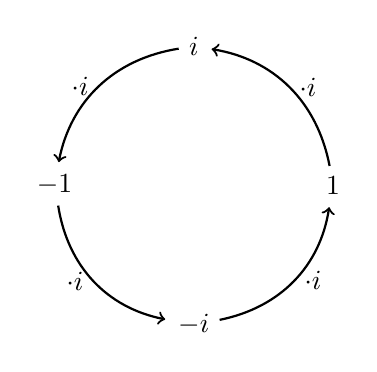
\begin{tikzpicture}[->,shorten >=1pt,auto,node distance=2.5cm,thick]
  \node (i) {$i$};
  \node (-1) [below left of=i] {$-1$};
  \node (-i) [below right of=-1] {$-i$};
  \node (1) [below right of=i] {$1$};
  \path [bend right=35]
  (i)  edge node [left]  {$\cdot i$} (-1)
  (-1) edge node [left] {$\cdot i$} (-i)
  (-i) edge node [right] {$\cdot i$} (1)
  (1) edge node [right] {$\cdot i$} (i);
\end{tikzpicture}
\end{center}

$$i^{4n}=1 \qquad i^{4n+1}=i \qquad i^{4n+2}=-1 \qquad i^{4n+3}=-i$$

\subsubsection*{Bijzondere machten}
\begin{align*}
  (a+bi)^0 &= 1\\
  (a+bi)^1 &= a+bi\\
  (a+bi)^2 &= a^2-b^2 + 2abi\\
  (a+bi)^3 &= (a^3 - 3ab^2) + (3a^2b -b^3)i\\
\end{align*}


\begin{oefening}
  Bereken
  \begin{enumerate}[(a)]
    \itemsep1em
  \item $\displaystyle \left(6+2i\right)^{-2}$
  \item $\displaystyle \left(1+2i\right)^4$
  \item $\displaystyle \dfrac{i^{35}+i^{40}}{1+i^{21}}$
  \item $\displaystyle \dfrac{(1+i)^2+(1-i)^2}{(1+i)^2-(1-i)^2}$
  \item $\displaystyle \left(\dfrac{1+i}{1-i}\right)^{30}+\left(\dfrac{1-i}{1+i}\right)^{30}$
  \end{enumerate}
\end{oefening}

\begin{oefening}
  Vereenvoudig
  \begin{enumerate}[(a)]
    \itemsep 1em
  \item $\frac{1+i}{1-i}-(1+2i)(2+2i)+\frac{3-i}{1+i}$;
  \item $2i(i-1)+\left(\overline{\sqrt{3}+i}\right)^3+(1+i)\overline{(1+i)}.$
  \end{enumerate}
\end{oefening}

\begin{oefening}
  We definiëren de {\bf positieve reële getallen} als $\mathbb{R}^+$. Dit zijn dus alle reële getallen met een positief teken, inclusief nul. We definiëren analoog de {\bf negatieve reële getallen} als $\mathbb{R}^-$. Dit zijn dus alle reële getallen met een negatief teken, inclusief nul.

  De positieve reële getallen en de negatieve reële getallen hebben dus het getal nul gemeenschappelijk:
  $$\mathbb{R}^+\cap\mathbb{R}^-=\{0\}$$

  {\bf Niet-positieve reële getallen} zijn dan alle reële getallen zonder de positieve reële getallen, {\bf niet-negatieve reële getallen} zijn dan alle reële getallen zonder de negatieve reële getallen.

  Als we een complex getal verschillend van nul vermenigvuldigen met zijn complex toegevoegde, dan krijgen we altijd een
  \begin{enumerate}[(A)]
  \item positief reëel getal.
  \item negatief reëel getal.
  \item niet-positief reëel getal.
  \item niet-negatief reëel getal.
  \end{enumerate}
\end{oefening}

\begin{oefening}*
Toon aan dat het getal
$$w=\dfrac{a}{a^2+b^2}-\dfrac{b}{a^2+b^2}i$$
de inverse voor de vermenigvuldiging is van het complex getal
$$z=a+bi\;.$$
\end{oefening}

\begin{oefening}
Bepaal $w$ zodat $(2+3i)\cdot w = 1$.
\end{oefening}

\begin{oefening}*
Bewijs volgende eigenschappen i.v.m. de complex toegevoegde van een complex getal:
\begin{enumerate}[a]
  \item $\overline{z+w}=\overline{z}+\overline{w}$
  \item $\overline{z\cdot w}=\overline{z}\cdot\overline{w}$
  \item $z\cdot\overline{z}\in\mathbb{R}$
\end{enumerate}
\end{oefening}

\begin{oefening}
Bepaal de macht $(a+bi)^4$.
\end{oefening}

\cleardoublepage
\section{Vierkantswortel van een complex getal}

\subsection{Definitie}
\begin{mdframed}
$x+yi$ is een {\bf vierkantswortel} uit $a+bi$ als en slechts als
\[(x+yi)^2 = a+bi\]
\end{mdframed}

\subsection{Voorbeelden}
\begin{enumerate}[(a)]
  \item $i$ is een vierkantswortel uit $-1$ want $i^2 = -1$
  \item $-3i$ is een vierkantswortel uit $-9$ want $(-3i)^2 = 9i^2 = -9$
  \item $3+i$ is een vierkantswortel uit $8+6i$ want $(3+i)^2=9+6i-1 = 8+6i$
\end{enumerate}

\subsection{Oplossingsmethode}

\subsubsection*{Voorbeeld 1}

Bepaal alle complexe getallen die een vierkantswortel zijn uit $3-4i$.

We zoeken dus $x+yi \in \mathbb{C}$, met $x,y\in\mathbb{R}$ zodat
\begin{align*}
  &&(x+yi)^2 &= 3-4i\\
  \lra &&\underbrace{x^2 - y^2}_{\text{\shortstack{reëel\\deel}}} + \underbrace{2xy}_{\text{\shortstack{imaginair\\deel}}}\hspace*{-0.3cm}i &= 3-4i\\
  \lra && &\hspace*{-2cm}\begin{cases}x^2 - y^2 = 3\\2xy =  -4 \mbox{ dus } x\neq 0 \wedge y\neq 0 \end{cases}\\
  \lra && &\hspace*{-2cm}\begin{cases}x^2 - y^2 = 3\\y =  -\frac{2}{x}\end{cases}\\
  \lra && &\hspace*{-2cm}\begin{cases}x^2 - \left(-\frac{2}{x}\right)^2 = 3\\y =  -\frac{2}{x}\end{cases}\\
  \lra && &\hspace*{-2cm}\begin{cases}x^2 - \frac{4}{x^2} = 3\\y =  -\frac{2}{x}\end{cases}\\
  \lra && &\hspace*{-2cm}\begin{cases}x^4-3x^2-4=0\\y =  -\frac{2}{x}\end{cases}
\end{align*}

In bovenstaand stelsel is $x^4-3x^2-4=0$ een {\bf bikwadratische vergelijking}. We lossen deze op m.b.v. een eenvoudige substitutie:
\begin{align*}
  &&\mbox{stel } t=x^2
  \Rightarrow t^2-3t-4&=0\\
  \lra && t^2-4t+t-4 &= 0\\
  \lra && (t-4)(t+1) &= 0\\
  \lra && t=4 \vee t=-1\\
  \lra && x^2=4 \vee \underbrace{\cancel{x^2=-1}}_{\text{want }x\in\mathbb{R}}
\end{align*}
Waardoor we nu ons stelsel verder kunnen oplossen:
\begin{align*}
  \lra && \begin{cases}x^2=4\\y=-\frac{2}{x}\end{cases}\\
  \lra && \begin{cases}x=2\\y=-\frac{2}{x}\end{cases} &&\vee&& \begin{cases}x=-2\\y=-\frac{2}{x}\end{cases}\\
  \lra && \begin{cases}x=2\\y=-1\end{cases} &&\vee&& \begin{cases}x=-2\\y=1\end{cases}
\end{align*}

We vinden dus twee oplossingen $x+yi\in\mathbb{C}$, namelijk
$$-2+i \mbox{ en } 2-i$$

Dus $3-4i$ heeft 2 vierkantswortels die elkaars tegengestelde zijn.

\subsubsection*{Voorbeeld 2}

Bepaal alle complexe getallen die een vierkantswortel zijn uit $-a$, met $a\in\mathbb{R}^+_0$.

We zoeken dus $z \in \mathbb{C}$, zodat
\begin{align*}
              && z^2 &= -a\\
         \lra && z^2 &= ai^2\\
         \lra && z   &= \pm \sqrt{ai^2}\\
         \lra && z   &= \pm \sqrt{a}\cdot i
\end{align*}

We vinden dus twee oplossingen $z\in\mathbb{C}$, namelijk
$$-\sqrt{a}i \mbox{ en } \sqrt{a}i$$

Dus $-a\in\mathbb{R}^+_0$ heeft 2 zuiver imaginaire wortels.


\begin{oefening}
  Bepaal alle vierkantswortels uit
  \begin{multicols}{2}
  \begin{enumerate}[(a)]
    \itemsep 1em
  \item $-9$
  \item $2i$
  \item $-3-4i$
  \item $-i$
  \end{enumerate}
\end{multicols}
\end{oefening}

\begin{oefening}
  Bepaal alle vierkantswortels uit
  \begin{multicols}{2}
  \begin{enumerate}[(a)]
    \itemsep 1em
  \item $(2i-3)(3-2i)$
  \item $i(1-i)$
  \item $\sqrt{2}-\sqrt{3}i$
  \item $i^5$
  \end{enumerate}
\end{multicols}
\end{oefening}

\cleardoublepage
\section{Vierkantsvergelijkingen in $\mathbb{C}$}

\subsection{Standaardvorm}

\begin{mdframed}
  Een vierkantsvergelijking in $\mathbb{C}$ is een vergelijking van de vorm
  \[az^2+bz+c=0 \text{ met } a\in\mathbb{C}_0, b,c\in\mathbb{C}\]
\end{mdframed}

Merk op: $a$ en $a$ zijn worden hier gezien als complexe coëfficiënten, en niet langer als een reëel deel en een imaginair deel.

\subsection{Eigenschap}

\begin{mdframed}
Elke vierkantsvergelijking
\[az^2+bz+c=0 \text{ met } a\in\mathbb{C}_0, b,c\in\mathbb{C}\]
heeft in $\mathbb{C}$ altijd twee (mogelijks samenvallende) oplossingen.
\end{mdframed}

\subsection{Voorbeelden}

\subsubsection*{Voorbeeld: Vierkantsvergelijking negatieve discriminant}

Los op in $\mathbb{C}$
$$z^2 + 2z + 5 = 0$$

\begin{align*}
  & a=1, b=2, c=5\\
  & \Rightarrow  D = b^2 - 4ac = -16\\
  & \Rightarrow  +\sqrt{D} = 4i \wedge -\sqrt{D}=-4i
\end{align*}

Dus we krijgen twee oplossingen:
\begin{align*}
  z_{1,2} &= \dfrac{-b \pm \sqrt{D}}{2a}\\
  \lra & \begin{cases}z_1 &= -1 - 2i\\z_2 &= -1 + 2i\end{cases}
\end{align*}

We noteren de oplossingenverzameling:
$$V=\{ -1-2i, -1+2i \}$$

\subsubsection*{Voorbeeld: Vierkantsvergelijking met imaginaire discriminant}

Los op in $\mathbb{C}$
\begin{align*}
       && (2-i)(z^2-6) &= 5(2i+1)z\\
  \lra && \underbrace{(2-i)}_a z^2 + \underbrace{(-5-10i)}_b z + \underbrace{(-12+6i)}_c &= 0
\end{align*}
\[\Rightarrow D = -3+4i\]


We willen nu $\sqrt{D}$ bepalen, m.a.w. we zoeken de wortels van $-3+4i$:
\begin{align*}
  &&(x+yi)^2 &= -3+4i\\
  \lra &&x^2 - y^2 + 2xyi &= -3+4i\\
  \lra && &\hspace*{-2cm}\begin{cases}x^2 - y^2 = -3\\2xy =  4 &\Rightarrow y=\frac{2}{x} \end{cases}\\
  \lra && &\hspace*{-2cm}\begin{cases}x^2 - \frac{4}{x^2} = -3\\y =  \frac{2}{x}\end{cases}\\
  \lra && &\hspace*{-2cm}\begin{cases}x^4+3x^2-4=0\\y =  \frac{2}{x}\end{cases}\\
  &&\mbox{stel } t=x^2
  \Rightarrow t^2+3t-4&=0\\
  \lra && t^2+4t-t-4 &= 0\\
  \lra && (t+4)(t-1) &= 0\\
  \lra && t=-4 \vee t=1\\
  \lra && \cancel{x^2=-4}\vee x^2=1\\
  \lra && \begin{cases}x=-1\\y=-2\end{cases} \vee \begin{cases}x=1\\y=2\end{cases}
\end{align*}

Dus vinden we $\sqrt{D} = -1-2i \mbox{ en } -\sqrt{D}=1+2i$. De oplossingen van onze vierkantsvergelijking worden dus
\begin{align*}
  z_{1,2} &= \dfrac{5+10i \mp (1+2i)}{2(2-i)}\\
  \lra & \begin{cases}z_1 &= \dfrac{(4+8i){\color{gray}(4+2i)}}{(4-2i){\color{gray}(4+2i)}}=2i\\z_2 &= 3i\end{cases}
\end{align*}

En dus de oplossingenverzameling wordt $V=\{2i, 3i\}$.

\subsection{Besluit}

\begin{mdframed}
De vierkantsvergelijking $az^2+bz+c=0$ met $a,b,c\in\mathbb{C}$ en $a\neq 0$ in $\mathbb{C}$ heeft als wortels
$$ z_{1,2}=\dfrac{-b\pm\sqrt{D}}{2a}$$
met $D=b^2-4ac$
\end{mdframed}

\begin{oefening}
  Los op in $\mathbb{C}$
  \begin{multicols}{2}
    \begin{enumerate}[(a)]
      \itemsep 1em
    \item $z^2-6z+10=0$
    \item $z^2+(i-5)z=7i-26$
    \item $z^2-4z+13=0$
    \item $iz^2+2z-13i-16=0$
    \item $z^2-4z+7+4i=0$
    \item $z^2+(i-4)z+5(1-i)=0$
    \item $z^2-(6+i)z+7+9i=0$
    \item $z^2-(1+i)z+(1+i)=0$
    \item $z^2-(4+2i)z+3+4i=0$
    \item $z^3-2z^2+(16+8i)z=0$
    \item $z^4+(1-4i)z^2=12+16i$
    \item $z^4+z^2+1=0$
    \item $z^4+(1-i)z^2-i=0$
    \item $z^4=(1+2i\sqrt{3})z^2+2+2i\sqrt{3}$
    \end{enumerate}
  \end{multicols}
\end{oefening}

\begin{oefening}
Los op in $\mathbb{C}$
  \begin{enumerate}[(a)]
    \itemsep 1em
  \item $5y+12=-\dfrac{8}{y}$
  \item $4+\dfrac{5}{x^2}=\dfrac{6}{x}$
  \item $\dfrac{3}{y-2}=\dfrac{1}{y}+1$
  \item $5z^2+2z=-1$
  \end{enumerate}
\end{oefening}

\pagebreak
\begin{oefening}*
  Bepaal $\lambda\in\mathbb{C}$ zodat
  \[iz^2+(\lambda-3i)z-2=0\]
  twee identieke wortels heeft.
\end{oefening}

\begin{oefening}*
De vierkantsvergelijking in $\mathbb{C}$
\[az^2+bz+c=0\]
met $a, b, c \in\mathbb{R}$ heeft ofwel twee (mogelijks samenvallende) reële oplossingen, ofwel twee complex oplossingen die elkaars toegevoegde zijn.
\end{oefening}

\begin{oefening}*
De vierkantsvergelijking in $\mathbb{C}$
\[z^2 + az + b = 0\]
met $a, b \in \mathbb{R}$ heeft zeker als oplossing
\[ z_1=2-i\;. \]
\begin{enumerate}[(a)]
  \item Bepaal de mogelijks andere oplossing.
  \item Bepaal de vierkantsvergelijking.
\end{enumerate}
\end{oefening}

\begin{oefening}*
Toon aan dat de vergelijking in $\mathbb{C}$
\[4z^3-6i\sqrt{3}z^2-3(3+i\sqrt{3})z+4=0\]
minstens één reële oplossing heeft.
\end{oefening}

\begin{oefening}*
Bepaal $z\in\mathbb{C}$ zodat
\[z^2+\overline{z}^2=0\;.\]
\end{oefening}

\cleardoublepage
\section{Vlak van Gauss}

\subsection{Meetkundige voorstelling van een complex getal}

$z=a+bi\in\mathbb{C}$ met $a,b\in\mathbb{R}$
\begin{itemize}
  \renewcommand{\labelitemi}{$\Rightarrow$}
  \item $z$ volledig bepaald door het koppel $(a,b)$
  \item $z$ in een assenstelsel voor te stellen als een punt $P(a,b)$
  \item met elke punt $P$ in dit vlak kan een complex getal $z$ voorgesteld worden
\end{itemize}

\begin{minipage}{.5\textwidth}
\begin{center}
\begin{tikzpicture}[scale=1.5,line cap=round,line join=round,>=triangle 45,x=1.0cm,y=1.0cm]
\draw[->,color=black] (-1.14,0) -- (3.74,0);
\foreach \x in {1}
\draw[shift={(\x,0)},color=black] (0pt,2pt) -- (0pt,-2pt) node[below] {\footnotesize $\x$};
\draw[->,color=black] (0,-0.72) -- (0,2.2);
\foreach \y in {1}
\draw[shift={(0,\y)},color=black] (2pt,0pt) -- (-2pt,0pt) node[left] {\footnotesize $\y$};
\draw[color=black] (-8pt,-5pt) node[right] {\footnotesize $0$};
\clip(-1.14,-0.72) rectangle (3.74,2.2);
\draw[color=black,fill=black,fill opacity=0.1] (0.21,0) -- (0.21,0.21) -- (0,0.21) -- (0,0) -- cycle;
\draw [line width=1.6pt] (0,1.5) -- (2.5,1.5);
\draw [line width=1.6pt] (2.5,0) -- (2.5,1.5);
\draw (2.3,-0.05) node[anchor=north west] {$a$};
\draw (-0.35,1.7) node[anchor=north west] {$b$};
\draw (2.63,1.74) node[anchor=north west] {$P(a,b)$};
\begin{scriptsize}
\fill [color=black] (2.5,1.5) circle (1.5pt);
\draw[color=black] (0.32,0.31) node {$90\degree$};
\end{scriptsize}
\end{tikzpicture}
\end{center}
\end{minipage}
\begin{minipage}{.5\textwidth}
Werk in een positief georiënteerd orthonormaal assenstelsel. Positief georiënteerd wil zeggen dat we de assen in tegenwijzerzin plaatsen. Orthonormaal wil zeggen dat de assen loodrecht op elkaar staan en dat ijking van alle assen gelijk is.
\end{minipage}

\subsection{Definitie}

\begin{mdframed}
Het vlak voorzien van een positief georiënteerd orthonormaal assenstelsel en waarvan elk punt beschouwd wordt als het beeldpunt van een complex getal noemen we het {\bf vlak van Gauss} of het complexe vlak.
\end{mdframed}

\begin{itemize}
  \item Op de $x$-as komen de reële getallen, we noemen dit dan ook de {\bf reële as} en noteren $Re$.
  \item Op de $y$-as komen de zuiver imaginaire getallen, we noemen dit dan ook de {\bf imaginaire as} en noteren $Im$.
\end{itemize}

\subsection{Voorbeelden}

Beschouw $z=a+bi\in\mathbb{C}$ en zijn beeldpunt $P(a,b)$

\begin{itemize}
  \item $z=0 \lra z=0+0i \lra P=$ oorsprong
  \item $z=a \lra P\in $ $x$-as = reële as
  \item $z=bi \lra P\in $ $y$-as = imaginaire as
  \item $z=a+bi \text{ met } P(a,b)$ en $\overline{z}=a-bi \text{ met } P'(a,-b)$\\
  $\Rightarrow$ $P$ en $P'$ zijn elkaars spiegelbeeld t.o.v. de $x$-as
  \item $z=a+bi \text{ met } P(a,b)$ en $-z=-a-bi \text{ met } P'(-a,-b)$\\
  $\Rightarrow$ $P$ en $P'$ zijn elkaars spiegelbeeld t.o.v. de oorsprong
\end{itemize}

\vspace*{1cm}
\begin{mdframed}% bron: http://www.promath.nl/wiskav04html/het_vlak_van_gauss.htm
{\em Wat http://www.promath.nl te zeggen heeft over het vlak van Gauss:}

Na Bombelli hebben veel wiskundigen zich op de een of andere manier bezig gehouden met complexe getallen. Toch blijven deze merkwaardige getallen lange tijd omgeven door een waas van onwerkelijkheid. Hoewel men steeds meer het nut inziet van het rekenen ermee blijft het complexe getal iets dat in werkelijkheid niet bestaat.

In het begin van de zeventiende eeuw, wanneer de negatieve getallen steeds nadrukkelijker geaccepteerd worden in de algebra, ontstaat het idee van een grafische weergave van getallen door middel van een getallenlijn. Reeds in het wiskundige werk van raadspensionaris Jan de Wit (1629-1672) treffen we het gebruik van twee onderling loodrechte getallenlijnen aan (coördinaatassen) om getallenparen weer te geven.

Nu kennen complexe getallen nog een extra complicatie, namelijk dat er feitelijk geen ordening van klein naar groot voor bestaat. Deze bestaat wel voor reële getallen en desnoods ook voor zuiver imaginaire getallen. Wallis komt als eerste met het idee om zuiver imaginaire getallen weer te geven op een getallenlijn die loodrecht op de reële getallenlijn staat. Het duurt echter nog ruim een eeuw tot de vrij onbekende Noor Caspar Wessel op het idee komt om het complexe getal als een soort getallenpaar in dit assenstelsel weer te geven. Zijn idee wordt gepubliceerd in een uitgave van 1798 van de Deense wiskundige academie. En pas als enige tientallen jaren later de grote wiskundige Carl Friedrich Gauss (1777-1855) dit idee in zijn werk gebruikt, wordt het algemeen overgenomen. De weergave van een complex getal in dit zogenaamde vlak van Gauss spreekt zo sterk tot de verbeelding, dat de resterende taboes rond de complexe getallen spoedig wegvallen. Nu er een grafische weergave bestaat, bestaat de complexe getallen zelf gewoon ook.
\end{mdframed}


\begin{oefening}
Stel volgende complexe getallen voor in het vlak van Gauss. Gebruik voor het complex getal $z_i$ het beeldpunt $P_i$.
$$z_1=5 \qquad z_2=1+i \qquad  z_3=2i \qquad  z_4=-2$$
$$z_5=-5+2i \qquad  z_6=3-4i \qquad  z_7=-3i \qquad  z_8=-i-2$$
\end{oefening}

\begin{oefening}
Bepaal de complexe getallen $z_i$ waarvan we in het vlak van Gauss de beeldpunten $P_i$ krijgen.
\begin{center}
\definecolor{cqcqcq}{rgb}{0.75,0.75,0.75}
\begin{tikzpicture}[line cap=round,line join=round,>=triangle 45,x=1.0cm,y=1.0cm]
\draw [color=cqcqcq,dash pattern=on 2pt off 2pt, xstep=1.0cm,ystep=1.0cm] (-3.92,-3.31) grid (4.93,3.65);
\draw[->,color=black] (-3.92,0) -- (4.93,0);
\foreach \x in {-3,-2,-1,1,2,3,4}
\draw[shift={(\x,0)},color=black] (0pt,2pt) -- (0pt,-2pt) node[below] {\footnotesize $\x$};
\draw[->,color=black] (0,-3.31) -- (0,3.65);
\foreach \y in {-3,-2,-1,1,2,3}
\draw[shift={(0,\y)},color=black] (2pt,0pt) -- (-2pt,0pt) node[left] {\footnotesize $\y$};
\draw[color=black] (0pt,-10pt) node[right] {\footnotesize $0$};
\clip(-3.92,-3.31) rectangle (4.93,3.65);
\draw (4.23,0.63) node[anchor=north west] {Re};
\draw (0.17,3.53) node[anchor=north west] {Im};
\begin{scriptsize}
\fill [color=black] (-2,2) circle (2.0pt);
\draw[color=black] (-1.74,2.25) node {$P_1$};
\fill [color=black] (0,1) circle (2.0pt);
\draw[color=black] (0.26,1.25) node {$P_2$};
\fill [color=black] (3,0) circle (2.0pt);
\draw[color=black] (3.25,0.25) node {$P_3$};
\fill [color=black] (-1,-3) circle (2.0pt);
\draw[color=black] (-0.74,-2.75) node {$P_5$};
\fill [color=black] (3,1) circle (2.0pt);
\draw[color=black] (3.25,1.25) node {$P_4$};
\end{scriptsize}
\end{tikzpicture}
\end{center}
\end{oefening}

\cleardoublepage
\section{Goniometrische gedaante van een complex getal}

\subsection{Modulus en argument van een complex getal}

\subsubsection*{Grafisch}

We stellen nu het beeldpunt $P(a,b)$ van een complex getal $z=a+bi \in \mathbb{C}$ anders voor:
\begin{itemize}
  \item door de {\em afstand} $|OP|=r$
  \item door de {\em hoek} $\phi$ tussen het positieve been van de reële as $Re$ en de halfrechte $OP$
\end{itemize}

\begin{center}
\definecolor{cqcqcq}{rgb}{0.75,0.75,0.75}
\begin{tikzpicture}[scale=2,line cap=round,line join=round,>=triangle 45,x=1.0cm,y=1.0cm]
\draw[->,color=black] (-1.35,0) -- (3.83,0);
\foreach \x in {1}
\draw[shift={(\x,0)},color=black] (0pt,2pt) -- (0pt,-2pt) node[below] {\footnotesize $\x$};
\draw[->,color=black] (0,-0.46) -- (0,2.12);
\foreach \y in {1}
\draw[shift={(0,\y)},color=black] (2pt,0pt) -- (-2pt,0pt) node[left] {\footnotesize $\y$};
\draw (3.6,-0.05) node[anchor=north west] {$Re$};
\draw (-0.5,2.2) node[anchor=north west] {$Im$};
\draw[color=black] (0pt,-5pt) node[left] {\footnotesize $0$};
\clip(-1.35,-0.46) rectangle (3.83,2.12);
\draw [shift={(0,0)},fill=black,fill opacity=0.1] (0,0) -- (0:0.28) arc (0:30.96:0.28) -- cycle;
\draw [line width=1.6pt] (0,0)-- (2.5,1.5);
\draw [line width=1.2pt,dash pattern=on 2pt off 2pt] (2.5,1.5)-- (2.5,0);
\draw [line width=1.2pt,dash pattern=on 2pt off 2pt] (2.5,1.5)-- (0,1.5);
\draw (2.6,1.72) node[anchor=north west] {$z=a+bi$};
\draw (2.4,-0.05) node[anchor=north west] {$a$};
\draw (-0.3,1.65) node[anchor=north west] {$b$};
\draw (1.07,0.94) node[anchor=north west] {$r$};
\fill [color=black] (2.5,1.5) circle (1.5pt);
\draw[color=black] (0.45,0.13) node {$\phi$};
\end{tikzpicture}
\end{center}

\subsubsection*{Definitie}
\begin{mdframed}
\begin{itemize}
  \item de afstand $r=|z|$ noemen we de {\bf modulus} van het complex getal $z$
  \item de hoek $\phi=\arg z$ noemen we een {\bf argument} van het complex getal $z$, deze hoek heeft oneindig veel waarden want
  $$\phi = \phi + k\cdot 360\degree \mbox{ met } k\in\mathbb{Z}$$
  Wij gebruiken steeds de hoofdwaarde van $\arg z$, namelijk het argument waarvoor geldt
  $0\degree \leq \arg z < 360\degree$
\end{itemize}
\end{mdframed}

\subsubsection*{Eigenschappen}
\begin{itemize}
  \item Het punt $P$ is ondubbelzinnig bepaald door $r$ en $\phi$ van $z$:
  $$z_1=z_2 \lra r_1=r_2 \wedge \phi_1=\phi_2$$
  \item $r\in\mathbb{R}^+$
  \item $z=0 \Rightarrow r=0 $ en $\phi$ is onbepaald
  \item $z$ en $\overline{z}$: gelijke moduli en tegengestelde argumenten
  \item $z$ en $-z$: gelijke moduli en argumenten verschillen $180\degree$
\end{itemize}

\subsubsection*{Bijzondere gevallen}\mbox{}

\begin{minipage}{0.5\textwidth}
\begin{center}
\begin{tabular}{c|c|c}
  $z$ & $r=|z|$ & $\phi=\arg z$\\
\hline
  1   & 1         &   0\degree\\
  i   & 1         &  90\degree\\
 -1   & 1         & 180\degree\\
 -i   & 1         & 270\degree\\
\end{tabular}
\end{center}
\end{minipage}
\begin{minipage}{0.5\textwidth}
\vspace*{-0.3cm}
\begin{center}
\begin{tikzpicture}[scale=1.5,line cap=round,line join=round,>=triangle 45,x=1.0cm,y=1.0cm]
\draw[->,color=black] (-1.56,0) -- (1.68,0);
\foreach \x in {-1,1}
\draw[shift={(\x,0)},color=black] (0pt,2pt) -- (0pt,-2pt) node[below] {\footnotesize $\x$};
\draw[->,color=black] (0,-1.66) -- (0,1.71);
\foreach \y in {-1,1}
\draw[shift={(0,\y)},color=black] (2pt,0pt) -- (-2pt,0pt);
\clip(-1.56,-1.66) rectangle (1.68,1.71);
\draw (2pt,1) node[right] {$i$};
\draw (2pt,-1) node[right] {$-i$};
\draw (0,1.5) node[left] {$Im$};
\draw (1.5,0) node[below] {$Re$};
\end{tikzpicture}
\end{center}
\end{minipage}

\subsection{Berekening van modulus en argument}

\subsubsection*{Gegeven:} $z=a+bi$

\subsubsection*{Gevraagd:} $r?\qquad \phi?$

\subsubsection*{Oplossing:}\mbox{}\\
\begin{minipage}{0.5\textwidth}
\begin{center}
\definecolor{cqcqcq}{rgb}{0.75,0.75,0.75}
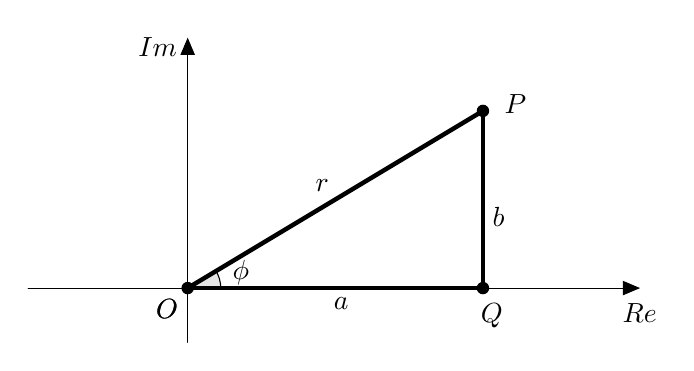
\begin{tikzpicture}[scale=1.5,line cap=round,line join=round,>=triangle 45,x=1.0cm,y=1.0cm]
\draw[->,color=black] (-1.35,0) -- (3.83,0);
\draw[->,color=black] (0,-0.46) -- (0,2.12);
\draw (3.6,-0.05) node[anchor=north west] {$Re$};
\draw (-0.5,2.2) node[anchor=north west] {$Im$};
\draw[color=black] (0pt,-5pt) node[left] {$O$};
\clip(-1.35,-0.46) rectangle (3.83,2.12);
\draw [shift={(0,0)},fill=black,fill opacity=0.1] (0,0) -- (0:0.28) arc (0:30.96:0.28) -- cycle;
\draw [line width=1.6pt] (0,0)-- (2.5,1.5);
\draw [line width=1.6pt] (2.5,1.5)-- (2.5,0);
\draw [line width=1.6pt] (2.5,0)-- (0,0);
\draw[color=black] (0pt,-5pt) node[left] {$O$};
\draw (2.6,1.72) node[anchor=north west] {$P$};
\draw (2.4,-0.05) node[anchor=north west] {$Q$};
\draw (1,1) node[anchor=north west] {$r$};
\draw (2.5,0.6) node[right] {$b$};
\draw (1.3,0) node[below] {$a$};
\fill [color=black] (2.5,1.5) circle (1.5pt);
\fill [color=black] (2.5,0) circle (1.5pt);
\fill [color=black] (0,0) circle (1.5pt);
\draw[color=black] (0.45,0.13) node {$\phi$};
\end{tikzpicture}
\end{center}
\end{minipage}
\begin{minipage}{0.5\textwidth}
In de rechthoekige driehoek $OPQ$ geldt:
\begin{itemize}
  \item wegens de stelling van Pythagoras dat $r^2=a^2+b^2$ en we weten dat $r\in\mathbb{R}^+$\\
  \framebox{$\Rightarrow r=\sqrt{a^2+b^2}$}\\
  \item $\begin{cases}a&=r\cos\phi\\b&=r\sin\phi\end{cases}$ zodat $\tan \phi = \dfrac{b}{a}$\\
  \framebox{$\Rightarrow\phi=\tan^{-1}\dfrac{b}{a}$}
\end{itemize}
\end{minipage}

\subsubsection*{Opmerkingen}
\begin{itemize}
  \item Dit geeft ons twee resultaten, we zullen moeten kijken in welk kwadrant $P(a,b)$ ligt om te weten welke oplossing de juiste is.
  \item Dit is niet geldig voor zuiver imaginaire getallen ($a=0$), maar in dat geval is $\phi=90\degree$ ($b>0$) of $\phi=-90\degree$ ($b<0$).
\end{itemize}

\subsection{Omgekeerde berekening}

\subsubsection*{Gegeven: } $r, \phi$

\subsubsection*{Gevraagd: } $z=a+bi$

\subsubsection*{Oplossing: }
\begin{itemize}
  \item $\cos \phi = \dfrac{a}{r}$ \; \framebox{ $\Rightarrow a=r\cos\phi$}
  \item $\sin \phi = \dfrac{b}{r}$ \; \framebox{ $\Rightarrow b=r\sin\phi$}
\end{itemize}

\subsection{Goniometrische gedaante}

Voorgaande resultaten kunnen we gebruiken om complexe getallen te schrijven in een andere vorm:
$$z = \underbrace{a+bi}_{\text{\shortstack{Carthesische\\vorm}}} = \underbrace{r(\cos\phi + i\sin\phi)}_{\text{\shortstack{Goniometrische\\vorm}}}$$

We noemen deze schrijfwijze de {\bf goniometrische vorm} of {\bf polaire vorm} van een complex getal. Het koppel $(r,\phi)$ noemen we de {\bf poolcoördinaten} van het punt $z$.

\begin{oefening}
Bepaal de goniometrische vorm, dus de vorm $z=r(\cos(\Phi)+i\sin(\Phi))$
\begin{multicols}{2}
\begin{enumerate}[(a)]
  \itemsep.5em
  \item $\displaystyle z=-1-i$
  \item $\displaystyle z=3i$
  \item $\displaystyle z=-2$
  \item $\displaystyle z=12-5i$
  \item $\displaystyle z=24-7i$
  \item $\displaystyle z=\cos(\alpha)-i\sin(\alpha)$
  \item $\displaystyle z=i-3$
  \item $\displaystyle z=-3i+4i-1$
  \item $\displaystyle z=\left(3+4i\right)^2$
  \item $\displaystyle z=9\cos(30\degree)+9i\sin(-30\degree)$
  \item $\displaystyle z=\dfrac{5+9i}{i}$
\end{enumerate}
\end{multicols}
\end{oefening}

\begin{oefening}
Bepaal de Carthesische vorm, dus de vorm $z=a+bi$
\begin{enumerate}[(a)]
  \itemsep.5em
  \item $\displaystyle z=2\left(\cos(45\degree)+i\sin(45\degree)\right)$
  \item $\displaystyle z=5\left(\cos(90\degree)+i\sin(90\degree)\right)$
  \item $\displaystyle z=12\left(\cos(180\degree)+i\sin(180\degree)\right)$
  \item $\displaystyle z=\pi\cdot\left(\cos(67\degree)+i\sin(247\degree)\right)$
  \item $\displaystyle z=\dfrac{13}{2}\cos(120\degree)+i\sin(120\degree)$
\end{enumerate}
\end{oefening}

\cleardoublepage
\section{Bewerkingen m.b.v. de goniometrische gedaante}

\subsection{Product}

Stel
\begin{align*}
  z_1 &= r_1 ( \cos \phi_1 + i \sin \phi_1 )\\
  z_2 &= r_2 ( \cos \phi_2 + i \sin \phi_2 )
\end{align*}

Dan berekenen we het product
\begin{align*}
  z_1 \cdot z_2 &= r_1 ( \cos \phi_1 + i \sin \phi_1 ) \cdot r_2 ( \cos \phi_2 + i \sin \phi_2 )\\
            &= r_1 r_2 (\cos \phi_1 \cos \phi_2 - \sin \phi_1 \sin \phi_2 + i ( \cos \phi_1 \sin \phi_2 + \sin \phi_1 \cos \phi_2))\\
            &= r_1 r_2 (\cos (\phi_1 + \phi_2) + i \sin (\phi_1 + \phi_2))
\end{align*}

We besluiten dat als we twee complexe getallen vermenigvuldigen in hun goniometrische gedaante, dat we dan de moduli mogen vermenigvuldigen en de argumenten mogen optellen.\\

\begin{mdframed}
  \[
    z_1 \cdot z_2 = r_1 r_2 \left(\cos (\phi_1 + \phi_2) + i \sin (\phi_1 + \phi_2)\right)
  \]
\end{mdframed}

\subsubsection*{Voorbeelden}

\begin{enumerate}[(a)]
\item Vermenigvuldig $\sqrt{3} + i$ met $-1+\sqrt{3}i$:
  \begin{align*}
      &&       z_1 &= \sqrt{3} + i = 2(\cos 30\degree + i\sin 30\degree)\\
      &&       z_2 &= -1 + \sqrt{3}i = 2(\cos 120\degree + i\sin 120\degree)\\[1em]
    \Rightarrow && z_1 \cdot z_2 &= 2 \cdot 2 \cdot ( \cos( 30\degree + 120\degree ) + i\sin( 30\degree + 120\degree ) )\\
      &&           &= 4 (\cos 150\degree + i\sin 150\degree)\\
      &&           &= 4 \left( -\dfrac{\sqrt{3}}{2} + i \dfrac{1}{2} \right)\\
      &&           &= -2\sqrt{3} + 2i
  \end{align*}
\item
  \begin{align*}
    \left[3(\cos 20\degree + i\sin 20\degree)\right] \cdot \left[4(\cos 70\degree + i\sin 70\degree)\right]  &= 12 (\cos 90\degree + i\sin 90\degree)\\
                       &= 12i
  \end{align*}
\end{enumerate}

\subsubsection*{Opmerking}

Indien we reeds over de goniometrische vorm beschikken gaat deze methode snel.

\begin{oefening}
Bereken:
\begin{enumerate}[(a)]
  \itemsep.5em
  \item Vermenigvuldig $z_1=4\left(\cos(40\degree)+i\sin(40\degree)\right)$ met $z_2=\left(\cos(-50\degree)+i\sin(-50\degree)\right)$
  \item Vermenigvuldig $z_1=2\left(\cos(50\degree)+i\sin(50\degree)\right)$ met $z_2=8\left(\cos(10\degree)+i\sin(10\degree)\right)$
  \item Vermenigvuldig $z_1=6\left(\cos(80\degree)+i\sin(80\degree)\right)$ met $z_2=2\left(\cos(20\degree)+i\sin(20\degree)\right)$
  \item Vermenigvuldig $z_1=2\left(\cos(50\degree)+i\sin(50\degree)\right)$ met $z_2=8\left(\cos(-40\degree)+i\sin(-40\degree)\right)$
  \item Vermenigvuldig $z_1=-5\sqrt{2}+5\sqrt{2} \cdot i$ met $z_2=5\left(\cos(45\degree)+i\sin(45\degree)\right)$
\end{enumerate}
\end{oefening}

\subsection{Quotiënt}

Stel
\begin{align*}
  z_1 &= r_1 ( \cos \phi_1 + i \sin \phi_1 )\\
  z_2 &= r_2 ( \cos \phi_2 + i \sin \phi_2 )
\end{align*}

We zoeken het quotiënt
\[z=\dfrac{z_1}{z_2} \mbox{ met } z=r(\cos \phi + i\sin \phi)\]
Dit is echter equivalent met
\begin{align*}
  &\Leftrightarrow& z \cdot z_2 &= z_1\\
  &\Leftrightarrow& z_1 &= z \cdot z_2\\
  &\Leftrightarrow& r_1 &= r \cdot r_2          &\wedge&&  \phi_1 &= \phi + \phi_2 \qquad \mbox{\scriptsize(product in goniometrische vorm)}\\
  &\Leftrightarrow&   r &= \dfrac{r_1}{r_2} &\wedge&&  \phi &= \phi_1 - \phi_2\\
\end{align*}

We besluiten dat als we twee complexe getallen delen in hun goniometrische gedaante, dat we dan de moduli mogen delen en de argumenten mogen aftrekken.\\

\begin{mdframed}
  \[
    \dfrac{z_1}{z_2} = \dfrac{r_1}{r_2} \left(\cos (\phi_1 - \phi_2) + i \sin (\phi_1 - \phi_2)\right)
  \]
\end{mdframed}

\subsubsection*{Voorbeeld}

Deel $\sqrt{3} + i$ met $-1+\sqrt{3}i$:
  \begin{align*}
      &&       z_1 &= \sqrt{3} + i = 2(\cos 30\degree + i\sin 30\degree)\\
      &&       z_2 &= -1 + \sqrt{3}i = 2(\cos 120\degree + i\sin 120\degree)\\\\
    \Rightarrow && \dfrac{z_1}{z_2} &= \dfrac{2}{2} ( \cos( 30\degree - 120\degree ) + i\sin( 30\degree - 120\degree ) )\\
      &&           &= \cos(-90\degree) + i\sin(-90\degree)\\
      &&           &= -i
  \end{align*}

\begin{oefening}
Bereken:
\begin{enumerate}[(a)]
  \itemsep.5em
  \item Deel $z_1=6\left(\cos(80\degree)+i\sin(80\degree)\right)$ door $z_2=2\left(\cos(20\degree)+i\sin(20\degree)\right)$
  \item Deel $z_1=2\left(\cos(50\degree)+i\sin(50\degree)\right)$ door $z_2=8\left(\cos(-40\degree)+i\sin(-40\degree)\right)$
  \item Deel $z_1=-5\sqrt{2}+5\sqrt{2} \cdot i$ door $z_2=5\left(\cos(45\degree)+i\sin(45\degree)\right)$
  \item Deel $z_1=3\left(\cos(20\degree)+i\sin(20\degree)\right)$ door $z_2=4\left(\cos(70\degree)+i\sin(70\degree)\right)$
  \item Deel $z_1=2\left(\cos(50\degree)+i\sin(50\degree)\right)$ door $z_2=8\left(\cos(10\degree)+i\sin(10\degree)\right)$
\end{enumerate}
\end{oefening}

\subsection{Macht}

Stel
\[z = r (\cos \phi + i \sin \phi )\]

Berekenen nu de $n$-de macht van $z$ met $n\in\mathbb{N}$
\begin{align*}
  z^n &= z \cdot z \cdot \ldots \cdot z\\
      &= r (\cos \phi + i \sin \phi ) \cdot r (\cos \phi + i \sin \phi ) \cdot \ldots \cdot r (\cos \phi + i \sin \phi )\\
      &= r \cdot r \cdot \ldots \cdot r (\cos( \phi + \phi + \ldots + \phi ) + i \sin( \phi + \phi + \ldots + \phi ))\\
      &= r^n \left(\cos(n\phi) + i\sin(n\phi)\right)
\end{align*}

We besluiten dat we voor de $n$-de macht van een complex getal de $n$-de macht van de modulus van het grondtal en het $n$-voud van het argument van het grondtal mogen nemen.

\begin{mdframed}
  \[
    z^n = r^n \left(\cos(n\phi) + i\sin(n\phi)\right)
  \]
\end{mdframed}

\subsubsection*{Voorbeeld}

Bereken $z^{15}$ als $z=\sqrt{3} + i$.

We bepalen eerst de goniometrische vorm van $z$:
\begin{align*}
  z &= \sqrt{3} + i\\
    &= 2(\cos30\degree + i\sin30\degree)
\end{align*}

We bepalen nu op goniometrische manier de macht en vormen het antwoord om in Carthesische vorm.
\begin{align*}
  z^{15} &= 2^{15}(\cos(15 \cdot 30\degree) + i\sin(15 \cdot 30\degree))\\
         &= 32768(\cos(450\degree) + i\sin(450\degree))\\
         &= 32768(\cos(90\degree) + i\sin(90\degree))\\
         &= 32768i
\end{align*}

\subsubsection*{Opmerking}
We merken dat deze methode merkelijk sneller gaat dan de macht via distributiviteit te willen uitrekenen, ook al moeten we eerst van cartesische naar goniometrische vorm omvormen.


\begin{oefening}
Bereken:
\begin{multicols}{2}
\begin{enumerate}[(a)]
  \itemsep.5em
  \item $\displaystyle \left(-1+\sqrt{3} \cdot i\right)^6$
  \item $\displaystyle \left(-\sqrt{2}-i\sqrt{2}\right)^5$
  \item $\displaystyle \left(1+i\sqrt{3}\right)^4$
  \item $\displaystyle \left(\sqrt{7}-i\right)^4$
  \item $\displaystyle \left(2-2i\right)^7$
  \item $\displaystyle \left(\dfrac{\sqrt{2}}{2}-\dfrac{\sqrt{2}}{2}i\right)^4$
  \item $\displaystyle \dfrac{\left(1+i\sqrt{3}\right)^{13}}{\left(\sqrt{3}-i\right)^8}$
\end{enumerate}
\end{multicols}
\end{oefening}

\cleardoublepage
\section{Formule van de Moivre}

\subsubsection*{Stelling}
De {\bf formule van de Moivre} stelt dat er voor elk complex getal
\[z=r \cdot (\cos \phi + i\sin \phi)\]
en elke $n\in\mathbb{Z}$ geldt dat
\begin{mdframed}
  \[ \left( \cos \phi + i\sin \phi \right)^n = \cos( n\phi ) + i\sin( n\phi ) \]
\end{mdframed}

\subsubsection*{Bewijs}
\begin{align*}
     &&                        z^n &= z^n\\
  \Leftrightarrow && r^n \cdot (\cos \phi + i \sin \phi)^n &= r^n \cdot (\cos( n\phi ) + i\sin( n\phi ))\\
  \Leftrightarrow && (\cos \phi + i \sin \phi)^n &= \cos( n\phi ) + i\sin( n\phi )\\
\end{align*}

\subsubsection*{* Alternatief bewijs}
Als we mogen gebruik maken van de {\bf formule van Euler}, namelijk dat er geldt dat
\[e^{i\phi} = \cos\phi + i\sin\phi \]
dan volgt {\em de Moivre} uit macht van een macht want
\begin{align*}
     && \left(e^{i\phi}\right)^n &= e^{in\phi}\\
  \Leftrightarrow && (\cos \phi + i \sin \phi)^n &= \cos( n\phi ) + i\sin( n\phi )\\
\end{align*}

Deze stelling legt een verbinding tussen de complexe getallen en de goniometrie!

\subsubsection*{Voorbeeld}

Bepaal de verdubbelingsformules.

\begin{align*}
  \cos 2\phi + i \sin 2\phi &= (\cos \phi + i \sin \phi)^2\\
                      &= \cos^2 \phi + 2i\cos\phi\sin\phi + i^2\sin^2\phi\\
                      &= \cos^2\phi - \sin^2\phi + 2i\cos\phi\sin\phi
\end{align*}

Er geldt dus
\[ \underbrace{\cos 2\phi}_{\text{reëel deel}} \;+ \;i \cdot \underbrace{\sin 2\phi}_{\text{imaginair deel}}
  = \underbrace{\cos^2\phi - \sin^2\phi}_{\text{reëel deel}} \; + \; i \cdot \underbrace{2\cos\phi\sin\phi}_{\text{imaginair deel}} \]

Reële delen en imaginaire delen gelijk stellen geeft ons
\[
  \begin{cases}
    \cos 2\phi &= \cos^2\phi - \sin^2\phi \\
    \sin 2\phi &= 2 \cos\phi \sin\phi
  \end{cases}
\]

\begin{oefening}
  Toon volgende goniometrische identiteiten aan:
  \begin{itemize}
  \item $\cos(4\phi) = \cos^4\phi - 6 \cos^2\phi \sin^2\phi + \sin^4\phi $
  \item $\sin(4\phi) = 4\cos^3\phi \sin\phi - 4 \cos\phi \sin^3\phi $
  \end{itemize}
\end{oefening}

\cleardoublepage
\section{Machtswortels zoeken m.b.v. de goniometrische gedaante}

\subsection{Definitie}

We noemen een complex getal $\omega$ een $n$-de machtswortel uit een complex getal $z$ als er geldt
\[\omega^n = z\]

\subsection{Methode}

\subsubsection*{Gegeven}
\[z=a+bi\]
of in goniometrische vorm
\[z=r(\cos\phi + i\sin\phi)\]

\subsubsection*{Gevraagd}
Alle $n$-de machtswortels uit $z$.

\subsubsection*{Oplossing}
Neem een willekeurige $n$-de wortel
\[\omega = \chi ( \cos \psi + i \sin \psi ) \]
We vinden dus $\omega$ als we de waarden voor $\chi\in\mathbb{R}$ en $\psi\in[0\degree,360\degree[$ vinden.

Omdat $\omega$ een $n$-de machtswortel van $z$ is geldt er
\begin{align*}
       & \quad \omega^n = z\\
  \Leftrightarrow \qquad & \begin{cases} \chi^n = r\\ n\psi = \phi + k \cdot 360\degree \qquad k\in\mathbb{Z} \end{cases}
\end{align*}

Er geldt dus
\begin{mdframed}
  \begin{align*}
    \chi &= \sqrt[n]{r}\\
    \psi &= \dfrac{\phi + k \cdot 360\degree}{n} \qquad k\in\mathbb{Z}
  \end{align*}
\end{mdframed}

\subsection{Algemeen}

Als een complex getal $z$ de goniometrische vorm
\[ z = r ( \cos \phi + i \sin \phi )\]
heeft, dan heeft $z$ precies $n\in\mathbb{N}_0$ verschillende $n$-de machtswortels, namelijk
\[ \omega_k = \sqrt[n]{r}\left( \cos\left( \dfrac{\phi + k \cdot 360\degree}{n} \right) + i \cdot \cos\left( \dfrac{\phi + k \cdot 360\degree}{n} \right) \right)\]
met $k = 0, 1, 2, \cdots , n-1$.

\subsubsection*{Opmerking}
\begin{itemize}
\item Een complex getal $>0$ bezit $n$ $n$-de wortels.
\item Deze $n$-de machtswortels kunnen worden voorgesteld in het vlak van Gauss, we bekomen dan de hoekpunten van een regelmatige $n$-hoek.
\end{itemize}

\subsection{Voorbeeld}

Bepaal alle $3$-de machtswortels uit 1 en stel ze grafisch voor in het vlak van Gauss.

\begin{align*}
  n &= 3\\
  z &= 1 \Rightarrow r = 1, \quad \phi = 0\degree\\
  \chi &= \sqrt[3]{1} = 1\\
  \psi &= \dfrac{0\degree + k \cdot 360\degree}{3} = k \cdot 120\degree \qquad k\in\mathbb{Z}
\end{align*}

Voor elke $k=0, 1, 2$ bepalen we nu de oplossing:
\begin{align*}
  k=0 \qquad \psi_0 &= 0\degree   &\Rightarrow \omega_0 &= 1 \cdot (\cos 0\degree + i \cdot \sin 0\degree)\\
            &             &       &= 1\\
  k=1 \qquad \psi_1 &= 120\degree &\Rightarrow \omega_1 &= 1 \cdot (\cos 120\degree + i \cdot \sin 120\degree)\\
            &             &       &= -\dfrac{1}{2} + i \cdot \dfrac{\sqrt{3}}{2}\\
  k=2 \qquad \psi_2 &= 240\degree &\Rightarrow \omega_2 &= 1 \cdot (\cos 240\degree + i \cdot \sin 240\degree)\\
            &             &       &= -\dfrac{1}{2} - i \cdot \dfrac{\sqrt{3}}{2}\\
\end{align*}

Het getal $1$ bezit dus $3$ verschillende $3$-de machtswortels:
\[1 \qquad -\dfrac{1}{2} + i \cdot \dfrac{\sqrt{3}}{2} \qquad -\dfrac{1}{2} - i \cdot \dfrac{\sqrt{3}}{2}\]

We stellen ze nu nog grafisch voor:

\begin{minipage}{.6\linewidth}
\begin{center}
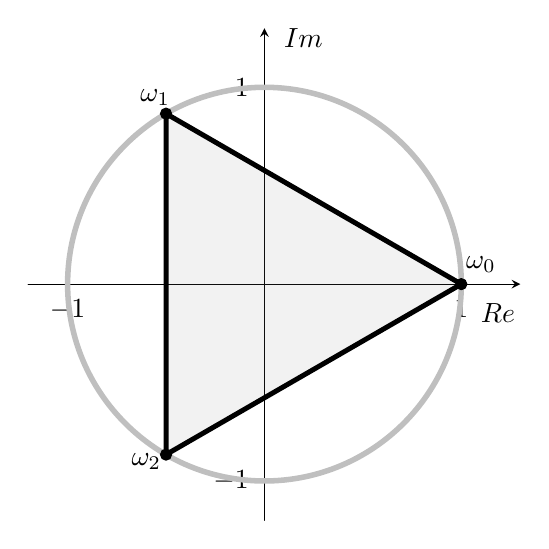
\begin{tikzpicture}[line cap=round,line join=round,>=triangle 45]
  \begin{axis}[scale=2.5,
    x=1.0cm,y=1.0cm,
    axis lines=middle,
    xmin=-1.2,
    xmax=1.3,
    ymin=-1.2,
    ymax=1.3,
    xtick={-1,0,1},
    ytick={-1,1}]
    \clip(-1.2,-1.2) rectangle (1.6,1.6);
    \draw[line width=1.8pt,color=black,fill=gray,fill opacity=0.1]
    (1.,0.) -- (-0.5,0.8660254037844386) -- (-0.5,-0.8660254037844386) -- cycle;
    \draw [line width=2.pt,color=lightgray] (0,0) circle (1);
    \begin{scriptsize}
      \draw (0.05,1.35) node[anchor=north west] {$Im$};
      \draw (1.05,-0.05) node[anchor=north west] {$Re$};
      \draw [fill=black] (1.,0.) circle (2pt);
      \draw (1.1,0.1) node {$\omega_0$};
      \draw [fill=black] (-0.5,0.8660254037844386) circle (2pt);
      \draw (-0.555,0.95) node {$\omega_1$};
      \draw [fill=black] (-0.5,-0.8660254037844386) circle (2pt);
      \draw (-0.6,-0.9) node {$\omega_2$};
    \end{scriptsize}
  \end{axis}
\end{tikzpicture}
\end{center}
\end{minipage}
\begin{minipage}{.4\linewidth}
  De beeldpunten van de 3 wortels in het vlak van Gauss vormen de hoekpunten van een gelijkzijdige driehoek.
\end{minipage}

\begin{oefening}
Bepaal alle
\begin{enumerate}[(a)]
  \itemsep.5em
  \item 4-de machtswortels uit $-2+i\sqrt{12}$
  \item 3-de machtswortels uit $2-2i$
  \item 5-de machtswortels uit $-\dfrac{\sqrt{2}}{2}-\dfrac{\sqrt{2}}{2}$
\end{enumerate}
\end{oefening}

\begin{oefening}
Beschouw het complex getal
$$-119-120i$$

\begin{enumerate}[(a)]
\item Bepaal alle vierde machtswortels uit bovenstaande getal. Rond, indien nodig, af op 2 decimalen. Gebruik de notatie $\omega_i$ waarbij je zelf de index $i$ kiest en zelf bepaalt hoeveel je er moet opschrijven.
\item Geef de beeldpunten van de wortels weer in het vlak van Gauss.
\item Welk een figuur vind je als je de beeldpunten verbindt?
\end{enumerate}
\end{oefening}

\subsection{Binomiale vergelijkingen}

% bron: LEERBOEK DER ALGEBRA VOOR H.B.S., GYMNASIUM EN LYCEUM, W.E.J.TJEENK WILLINK, ZWOLLE, 1937
Onder een {\bf binomiaalvergelijking} verstaat men een vergelijking van de $n$-de graad ($n~\geq~1$), waarvan het op nul herleide lid uit twee termen bestaat. De algemene gedaante van een binomiaal vergelijking is
\[az^n + bz^m=0\]

In onze context kunnen we veronderstellen dat de vorm herleidbaar is tot
\begin{align*}
     && az^n+b &= 0 \text{ met } a\in\mathbb{C}_0, b\in\mathbb{C}\\
  \Leftrightarrow &&    z^n  &= -\dfrac{b}{a}
\end{align*}

Als we nu $z$ en $-\dfrac{b}{a}$ uitdrukken in hun goniometrische vorm
\[z=r\cdot(cos\phi + i\sin\phi) \text{ en } -\dfrac{b}{a}=\chi \cdot ( \cos\psi + i\sin\psi )\]
dan is $z^n=-\dfrac{b}{a}$ oplossen equivalent met de $n$-de machtswortels bepalen m.b.v. de methode daarnet.

\subsubsection*{Voorbeeld}

Los de volgende vergelijking op in $\mathbb{C}$
\[2z^8-6z^3=0\]
\begin{align*}
     && 2z^8-6z^3 &= 0\\
  \Leftrightarrow && 2z^3 \cdot (z^5 - 3) &= 0\\
  \Leftrightarrow && 2z^3 = 0 \qquad &\vee \qquad z^5 - 3 = 0\\
\end{align*}
In $2z^3 = 0$ vinden we alvast drie oplossingen:
\[z_0 = 0 \quad z_1 = 0 \quad z_2 = 0\]
of kort
\[z_0 = z_1 = z_2 = 0\]

We bepalen nu nog de oplossingen van $z^5 - 3 = 0 \Leftrightarrow z^5 = 3$:
\begin{align*}
  z &= r(\cos\phi + i\sin\phi)\\
  3 &= 3(\cos0\degree + i\sin0\degree)\\
    &\Rightarrow \chi = \sqrt[5]{3}\\
    &\Rightarrow \psi = \dfrac{ 0\degree +  k360\degree }{ 5 } = k\cdot72\degree \qquad k\in{0, 1, 2, 3, 4}
\end{align*}
We vinden dus nog 5 oplossingen
\begin{align*}
  k=0 \qquad \psi_0 &= 0\degree   &\Rightarrow z_3=\omega_0 &= \sqrt[5]{3} \cdot (\cos 0\degree + i \cdot \sin 0\degree)\\
            &             &           &\approx 1.26\\
  k=1 \qquad \psi_1 &= 72\degree  &\Rightarrow z_4=\omega_1 &= \sqrt[5]{3} \cdot (\cos 72\degree + i \cdot \sin 72\degree)\\
            &             &           &\approx 0.38 + 1.18i\\
  k=2 \qquad \psi_2 &= 144\degree &\Rightarrow z_5=\omega_2 &= \sqrt[5]{3} \cdot (\cos 144\degree + i \cdot \sin 144\degree)\\
            &             &           &\approx -1.01 + 0.73i\\
  k=3 \qquad \psi_3 &= 216\degree &\Rightarrow z_6=\omega_3 &= \sqrt[5]{3} \cdot (\cos 216\degree + i \cdot \sin 216\degree)\\
            &             &           &\approx -1.01 - 0.73i\\
  k=4 \qquad \psi_4 &= 288\degree &\Rightarrow z_7=\omega_41 &= \sqrt[5]{3} \cdot (\cos 288\degree + i \cdot \sin 288\degree)\\
            &             &           &\approx 0.38 - 1.18i\\
\end{align*}

We vinden dus uiteindelijk de oplossingenverzameling
\[V=\{0, 1.26, 0.38 + 1.18i, -1.01 + 0.73i, -1.01 - 0.73i, 0.38 - 1.18i\}\]



\begin{oefening}
Los op in $\mathbb{C}$ en geef de oplossing grafisch weer in het vlak van Gauss.
\begin{multicols}{2}
\begin{enumerate}[(a)]
  \itemsep.5em
  \item $\displaystyle z^2=1+i\sqrt{3}$
  \item $\displaystyle z^4-64z = 0$
  \item $\displaystyle 4z^5+4i\sqrt{3}z^2=4z^2$
  \item $\displaystyle z^4+2-2i\sqrt{3}=0$
  \item $\displaystyle z^{10}+iz^5=0$
  \item $\displaystyle 8z^8+64z^2=0$
  \item $\displaystyle z^8-1=0$
\end{enumerate}
\end{multicols}

\begin{oefening}
  Beschouw de binomiale vergelijking in $\mathbb{C}$
$$z^3=8i$$
\begin{enumerate}[(a)]
\item Geef één mogelijke oplossing van bovenstaande vergelijking.
\item Hoeveel oplossingen zal bovenstaande vergelijking in het totaal hebben?
\item Gebruik deze informatie om de oplossingenverzameling grafisch weer te geven.
\item Teken in bovenstaande assenstelsel (in een ander kleur) ook de oplossingen van
  $$z^6=-64$$
\end{enumerate}
\end{oefening}

\end{oefening}

\appendix
\cleardoublepage
\section{Grieks alfabet}

\begin{center}
  \begin{tabular}{lcc}
    \hline
    \bf uitspraak & \bf klein & \bf groot \\
    \hline
    alfa & $\alpha$ & A\\
    bèta & $\beta$ & B\\
    gamma & $\gamma$ & $\Gamma$ \\
    delta & $\delta$ & $\Delta$ \\
    e-psilon & $\epsilon$ & E\\
    zèta & $\zeta$ & Z\\
    èta & $\eta$ & H\\
    thèta & $\theta$ of $\vartheta$ & $\Theta$\\
    jota & $\iota$ & I\\
    kappa & $\kappa$ & K\\
    lambda & $\lambda$ & $\Lambda$\\
    mu & $\mu$ & M\\
    nu & $\nu$ & N\\
    ksi & $\xi$ & $\Xi$\\
    o-mikron & $o$ & O\\
    pi & $\pi$ of $\varpi$ & $\Pi$\\
    ro & $\rho$ of $\varrho$ & P\\
    sigma & $\sigma$ of $\varsigma$ & $\Sigma$\\
    tau & $\tau$ & T\\
    u-psilon & $\upsilon$ & $\Upsilon$\\
    fi & $\phi$ of $\varphi$ & $\Phi$\\
    chi & $\chi$ & X\\
    psi & $\psi$ & $\Psi$\\
    o-mega & $\omega$ & $\Omega$\\
    \hline
  \end{tabular}
\end{center}


\end{document}
